\documentclass{standalone}

\usepackage{tikz}
\usetikzlibrary{angles,quotes}
\usepackage{amsmath,amssymb,amsfonts,xcolor}

\usepackage{pgfplots}
\definecolor{darkgreen}{rgb}{0.0, 0.42, 0.24}
\definecolor{amethyst}{rgb}{0.6, 0.4, 0.8}

\pgfplotsset{compat=newest}
\pgfplotsset{every axis/.append style={
                     tick label style={font=\footnotesize},
                 }}

\begin{document}
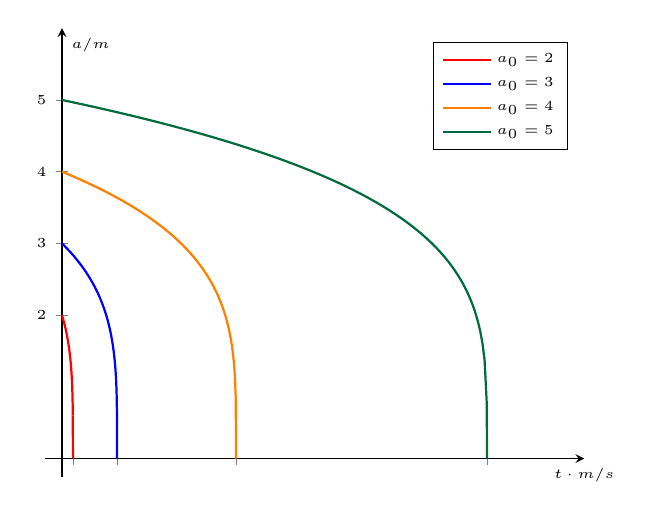
\begin{tikzpicture}
        \begin{axis}[xmin=-0.5,xmax=15,ymin=-0.25,ymax=6,
        axis lines = middle,
        xlabel=$t\cdot m/s$,
        ylabel=$a/m$,
        label style={font=\tiny},
        tick label style={font=\tiny},
        xtick={0.314,1.58,5,12.207},
        xticklabels={},
        xticklabel style={anchor=north},
        xlabel style={anchor=north},
        ytick={0,2,3,4,5},
        domain=0:15,
        restrict y to domain=-0.1:6,
        legend pos =north east,
        legend style={font=\tiny}]
            \addplot[color=red,samples=200,thick,domain=0:0.31]{(2^4-(256/5)*x)^0.25};
             
             
           \addplot[color=blue,samples=200,thick,domain=0:1.58]{(3^4-(256/5)*x)^0.25};
           
           
           \addplot[color=orange,samples=200,thick,domain=0:4.99]{(4^4-(256/5)*x)^0.25};
           
           \addplot[color=darkgreen,samples=200,thick,domain=0:12.2]{(5^4-(256/5)*x)^0.25};
           
           \addplot[color=darkgreen,thick,samples=3] coordinates {(12.2,0.775)(12.207,0)};
           \addplot[color=red,thick,samples=3] coordinates {(0.31,0.598)(0.314,0)};
           \addplot[color=blue,thick,samples=3] coordinates {(1.58,0.568)(1.582,0)};
           \addplot[color=orange,thick,samples=3] coordinates {(4.99,0.846)(5,0)};
           %\addplot[color=gray,dashed,samples=50,domain=4:20]{1/(6*(x-3))-2/(3*x)};
           \addlegendentry{$a_0=2$}
           \addlegendentry{$a_0=3$}
           \addlegendentry{$a_0=4$}
           \addlegendentry{$a_0=5$}
        \end{axis}
    \end{tikzpicture}
\end{document}